\documentclass[titlepage,11pt]{article}

\usepackage{amsmath, amssymb}
\usepackage{float}
\usepackage{gensymb}
\usepackage[pdftex]{graphicx}
\usepackage[margin=1in]{geometry}
\usepackage{ragged2e}
\usepackage{setspace}
\usepackage{cleveref}
\usepackage{siunitx}% si units
\usepackage{wrapfig}
\usepackage[utf8]{inputenc} % Required for inputting international characters
\usepackage[T1]{fontenc} % Output font encoding for international characters
\usepackage{mathpazo} % Palatino font
\usepackage{xcolor}
\usepackage[sort&compress,numbers,super]{natbib}
\usepackage{caption}
\usepackage{subcaption}
\usepackage{chngpage}

\newcommand{\figfile}{./figures}
\newcommand{\HOS}{{\color{red}HOS}}
\newcommand{\Ham}{\widehat{\mathcal{H}}}

\begin{document}
%----------------------------------------------------------------------------------------
%	TITLE PAGE
%----------------------------------------------------------------------------------------

\begin{titlepage} % Suppresses displaying the page number on the title page and the subsequent page counts as page 1
	\newcommand{\HRule}{\rule{\linewidth}{0.5mm}} % Defines a new command for horizontal lines, change thickness here
	
	\center % Centre everything on the page
	\begin{figure*}
		\centering
		\includegraphics[width=\textwidth]{figures/UBC_Chemlogo.eps}
	\end{figure*}
	
	
	%------------------------------------------------
	%	Headings
	%------------------------------------------------
	
	\textsc{\LARGE Fourth Year Meeting\\ \vspace{1em}  \& Thesis Outline}\\[1.5cm] % Main heading such as the name of your university/college
	
	
	%------------------------------------------------
	%	Title
	%------------------------------------------------
	
	\HRule\\[0.4cm]
	
	{\huge\bfseries Exploration of Crystal Nucleation Phenomena Through Molecular Simulation}\\[0.4cm] % Title of your document
	
	\HRule\\[1.5cm]
	
	%------------------------------------------------
	%	Author(s)
	%------------------------------------------------
	
	\begin{minipage}{0.4\textwidth}
		\begin{flushleft}
			\large
			\textit{Author}\\
			Hayden \textsc{Scheiber} % Your name
		\end{flushleft}
	\end{minipage}
	~
	\begin{minipage}{0.4\textwidth}
		\begin{flushright}
			\large
			\textit{Supervisor}\\
			Dr. Gren \textsc{Patey} % Supervisor's name
		\end{flushright}
	\end{minipage}\\

	\vspace{1cm}
	
	%\begin{minipage}{0.4\textwidth}
	%	\begin{flushleft}
	%		\large
	%		\textit{Chair}\\
	%		Dr. Geoffrey \textsc{Herring} % Chair
	%	\end{flushleft}
	%\end{minipage}
	~
	\begin{minipage}{0.4\textwidth}
		\begin{center}
			\large
			\textit{Committee}\\
			Dr. Yan \textsc{Wang}\\ % Committee
			Dr. Mark \textsc{Thachuk}\\ % Committee
			Dr. Keng \textsc{Chou} % Committee
		\end{center}
	\end{minipage}
	
	%------------------------------------------------
	%	Date
	%------------------------------------------------
	
	\vfill\vfill\vfill % Position the date 3/4 down the remaining page
	
	{\large
	\begin{table}[H]
		\centering
		\begin{tabular}{lll}
			\textbf{Date} & \textbf{Time} & \textbf{Location} \\
			Monday, October 4$^{\text{th}}$ 2021 & 11:00 AM & CHEM D317
		\end{tabular}
	\end{table}
	}
	%------------------------------------------------
	%	Logo
	%------------------------------------------------
	
	%\vfill\vfill
	%\includegraphics[width=0.2\textwidth]{placeholder.jpg}\\[1cm] % Include a department/university logo - this will require the graphicx package
	 
	%----------------------------------------------------------------------------------------
	
	\vfill % Push the date up 1/4 of the remaining page
	
\end{titlepage}

%----------------------------------------------------------------------------------------

%\large
\justifying
\doublespacing

\section{Introduction}

The theme of this thesis can best be described as a theoretical study of crystal energetics and crystal nucleation mechanisms~\cite{Karthika2016} in lithium halide (LiX) salts. For the first project in this thesis, we spent a considerable amount of time focusing on the relative energetics of different LiX crystal structures.~\cite{scheiber2021analysis} The goal of this first project was to determine why two of the most commonly employed LiX classical models~\cite{Fumi1964,Tosi1964,Joung2008} predict the wrong crystal structure of LiX in many cases, in particular for LiBr and LiI.

All projects following the first in this thesis depend strongly on the discoveries we made, and high-quality reference data we created, over the course of the first project. The second project employs Bayesian optimization~\cite{mockus2012bayesian} to efficiently search for classical model parameters that reproduce known experimental and density functional theory (DFT) targets. The methodology corresponds to a global optimization of a user-defined objective function through a high-dimensional parameter space on a predefined domain. With this methodology we explore the fundamental limitations of classical pairwise models, and produce useful models for lithium halide simulation which can simultaneously reproduce many known experimental and DFT results to useful accuracy, including the correct low-energy crystal structure.

Project 3 is a deep-dive into the physics behind why the NiAs crystal structure of LiI (and LiBr) is not observed experimentally, despite being a very low-energy state as determined by high accuracy DFT calculations. In project 4, we train neural networks to solve an molecular dynamics trajectory analysis problem: how to distinguish different phases of lithium halides during a phase-change event such as melting or crystallization. With project 5, which is not yet near completion, we aim to explore how LiX metastable wurtzite crystals can nucleate under certain experimental conditions.

\textbf{Expected date of thesis completion: end of August 2022.}

\section{Project 1: Analysis of the relative stability of lithium halide crystal structures: Density functional theory and classical models}

We spent a considerable amount of effort finding the best possible theoretical approach to study the energetics of (infinitely periodic) lithium halide crystal structures to the highest possible accuracy, while remaining computationally feasible, by employing state-of-the-art density functional theory methods with large basis sets. This is demonstrated in Figs.~\ref{fig:cp2k_EX_DeltaEExp} and~\ref{fig:cp2k_EX_DeltaAExp}. Along the way, we discovered that the relatively weak London dispersion interaction plays a critical role in determining the relative energetics of possible low-energy LiX crystal structures. In particular, the rocksalt structure, which is the thermodynamically stable crystal structure of all lithium halides under ambient conditions, is favoured over the closely-competing wurtzite crystal structure primarily due to second shell halide-halide dispersion interactions. In fact, dispersion-free Hartree-Fock calculations show that LiBr and LiI would both exist as wurtzite if it were not for dispersion.

By scaling up the strength of the halide-halide dispersion interaction in two existing simple pairwise classical models,~\cite{Fumi1964,Tosi1964,Joung2008} we could bring these models to energetically favour the experimental rocksalt structure at a modest cost of increased error in the total lattice energy and lattice parameter $a$ compared with experiment.

\textbf{Status: 100 \% complete.} This project is published in the journal of chemical physics\cite{scheiber2021analysis} and should occupy approximately one third of the total thesis.

\begin{figure}
	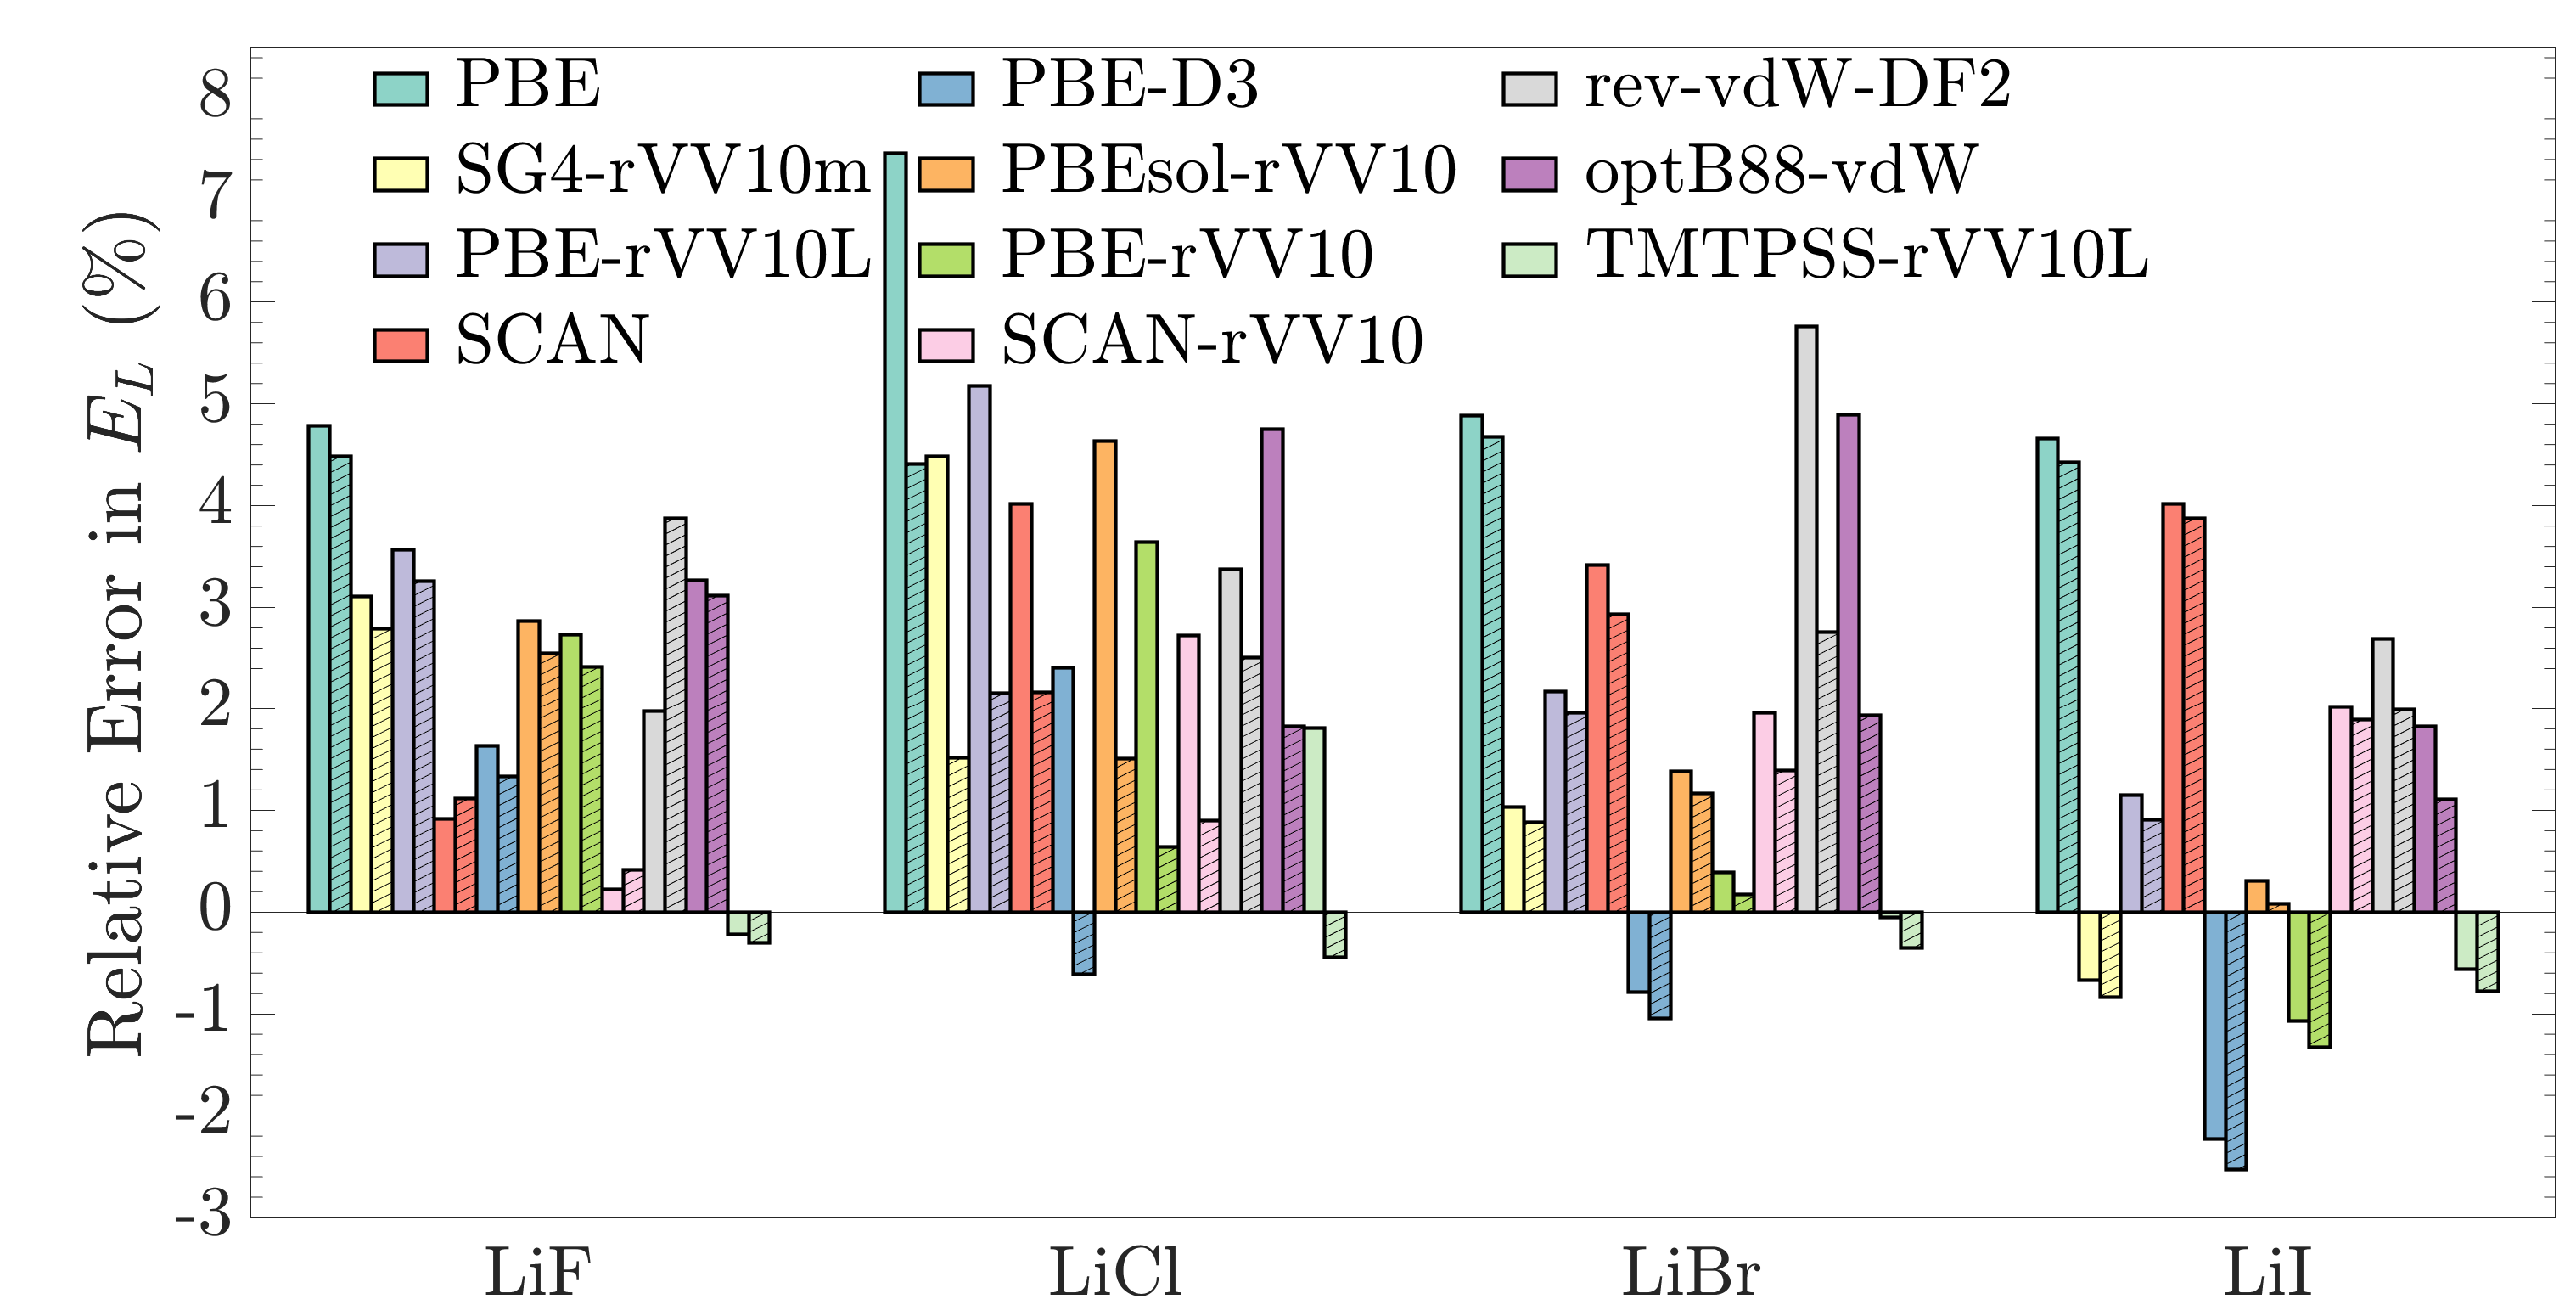
\includegraphics[width=\textwidth]{\figfile/fig_cp2k_EX_DeltaEExp.eps}
	\caption{\label{fig:cp2k_EX_DeltaEExp} The relative error ($[E_{L}(\text{Theory, Rocksalt}) - E_{L}(\text{Experiment}) ] / | E_{L}(\text{Experiment}) |$) in lattice energy for various quantum mechanical calculations. Use of the pob-TZVP basis set~\cite{Peintinger2013} (or Sapporo-DKH3-TZP~\cite{sekiya2001contracted,noro2009relativistic} for Br and I) for the crystal energies is indicated by solid bars, while hatched bars indicate the larger Sapporo-QZP (or Sapporo-DKH3-QZP for Br and I) basis set on the anions. The def2-TZVPD basis set~\cite{weigend2005balanced} for isolated ions corresponding to pob-TZVP, while diffuse augmented Sapporo basis sets are otherwise used. Scalar relativistic effects are included by a third order Douglas–Kroll–Hess transformation~\cite{douglas1974quantum,hess1985applicability,nakajima2012douglas} for all LiBr and LiI calculations. Theoretical lattice energies are those calculated from optimized rocksalt structures.}
\end{figure}

\begin{figure}
	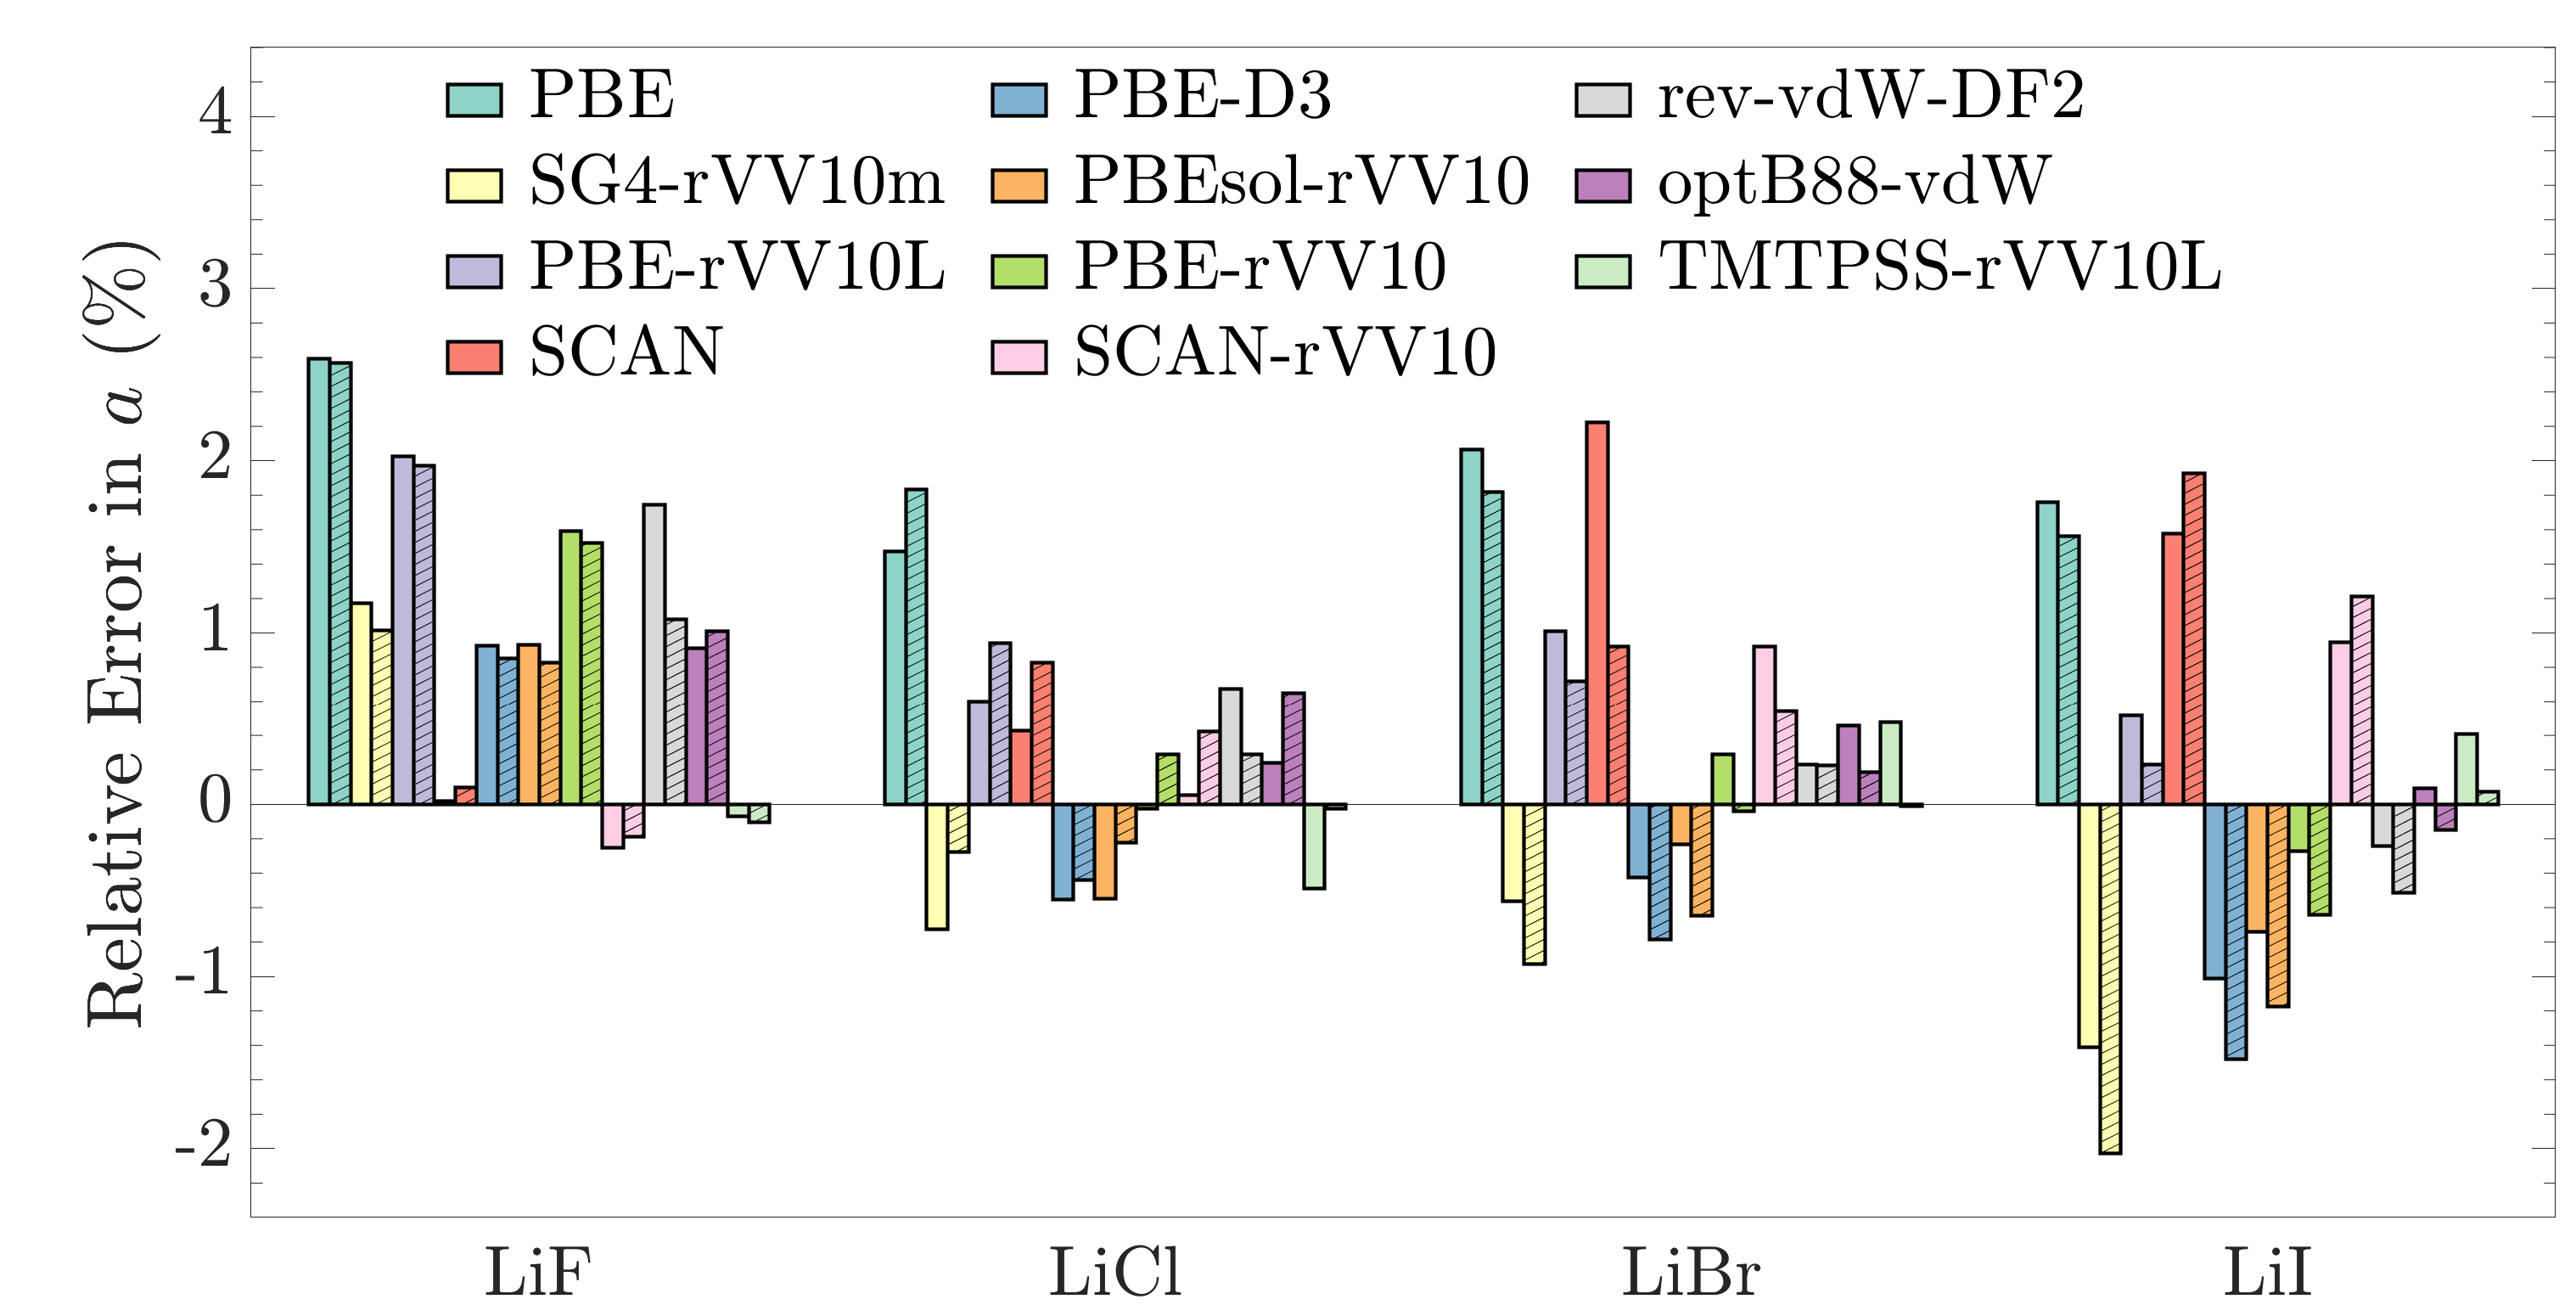
\includegraphics[width=\textwidth]{\figfile/fig_cp2k_EX_DeltaAExp.eps}
	\caption{\label{fig:cp2k_EX_DeltaAExp} The relative error ($(a_{\text{calculated}} - a_{\text{experiment}})/a_{\text{experiment}}$) in calculated lattice parameter $a$ for various quantum mechanical calculations. Use of the pob-TZVP basis set (or Sapporo-TZP for I) for the crystal energies is indicated by solid bars, while hatched bars indicate the larger Sapporo-QZP basis set on the anions. Theoretical lattice parameters are those from fully optimized rocksalt unit cells.}
\end{figure}



\section{Project 2: Bayesian Optimization for Lithium Halide Forcefields: Exploring the Limits of Pairwise Additive Potentials for Molecular Simulation}

Project two is a collaboration between three research groups an UBC. It derives from the first project, wherein we constructed a program to efficiently optimize the crystal structure of a lithium halide system given an input forcefield and initial unit cell. In project two, whose methodology is summarized in Fig.~\ref{fig:BO_Overview}, we push up one further level of abstraction, treating the crystal optimizer as part of a blackbox function with model parameters as inputs. Within the blackbox function, we pass the outputs of the crystal optimizer (lattice energies, relative lattice energies, and lattice parameters) into an objective function, using the set of experimental and DFT data from project 1 as targets. The lattice energies and lattice parameters corresponding to a set of input model parameters are taken with a subset of user-defined targets and weights. The input model energies and lattice parameters are used to calculate a linear combination of L2 losses based on the user-defined targets. This combined loss is the output of the objective function.

Since the blackbox functions are slow to calculate, taking up to 15 minutes for a parameter set to return a function value without any analytical gradients, Bayesian optimization is well-suited to optimize the input model parameters. We use this methodology to generate useful sets of parameters for simple pairwise models that reproduce experimental or DFT-calculated results of interest.

\begin{figure}
	\includegraphics[width=\textwidth]{\figfile/Bayesian_Optimization_Overview.pdf}
	\caption{\label{fig:BO_Overview} Overview of the methodology employed in project 2.}
\end{figure}

\textbf{Status: 90 \% complete.} All relevant project code, most data collection, and most data analysis is complete.


\section{Project 3: The NiAs Crystal Structure of LiI: Low Energy, but Never Observed}

This project combines aspects of both project 1 and project 2, again employing the high-quality reference data we produce in project 1 with the methodology from project 2. In this project, we use custom models created with the methodology of project 2 to explore why the NiAs crystal structure is not observed for LiI experimentally. Our highest-quality DFT results, shown in Fig.~\ref{fig:RS_NiAs_Compare} predict that at (T = 0, P = 0) the NiAs crystal structure is the energetically most stable structure of LiI, beating out rocksalt by $\SI{0.43}{\kilo\joule\per\mole}$. Despite this, there is to date no experimental evidence that the NiAs structure crystallizes in solid LiI. On the other hand, the higher-energy wurtzite crystal structure of LiI has been observed under certain experimental conditions.~\cite{vcanvcarevic2005theoretical}


\textbf{Status: 70 \% complete.} Relevant project code is complete and much of the data is collected. A few more simulations are required.


\begin{figure}
	\includegraphics[trim={0 0 0 0.1cm},clip,width=\textwidth]{\figfile/Rocksalt_NiAs_Components.png}
	\caption{\label{fig:RS_NiAs_Compare} A breakdown of the quantum-mechanical difference in energies between rocksalt and NiAs crystal structures ($\Delta E_{L} = E_{L}(\text{Rocksalt}) - E_{L}(\text{NiAs})$) for the four LiX salts, calculated at the TMTPSS-rVV10L~\cite{tao2016accurate,patra2019performance} level of theory with large, quadruple-zeta valence basis sets.~\cite{scheiber2021analysis} Positive energies favour NiAs while negative energies favour rocksalt. A purely Coulombic $\pm 1$ point charge model (Hard Spheres Coulombic) employing the DFT optimized geometries is included for comparison.}
\end{figure}


\section{Project 4: Convolutional Neural Networks with Steinhart Order Parameters: Machine Learning for Structure Detection in Molecular Simulation}

This project came out of the need to distinguish different lithium halide crystal structures in simulation. In a molecular dynamics simulation of LiX crystallization from a melt, it is not always obvious which structure has crystallized out. Additionally, it is usually not clear where the newly forming crystallite ends and the surrounding liquid begins. Steinhart Order Parameters~\cite{steinhardt1983bond} can be employed to distinguish different crystal structures, as well as distinguish liquids, but these are most often employed to distinguish only two competing phases. In the case of lithium halides, there exist up to six low-lying crystal structures competing for crystallization, plus the liquid phase.

To deal with the complexity of separating out the distinct order parameter signals of the seven possible LiX phases, we constructed a neural network for phase classification and trained it on the trajectories of multiple molecular dynamics simulations, at least one for each phase of interest. These reference molecular dynamics simulations were constructed to contain only one phase at a time over a range of temperature. This technique simplified the categorization of the reference trajectories.

The neural network uses multiple Steinhart Order Parameters as features: nine of them in total. These differ in the number of nearby atoms to consider (4, 6, or 18 nearest neighbours), as well as the order of the maximum spherical harmonic to use. It is only by employing multiple order parameters that we can reliably separate out the signatures of all six LiX crystal structures and the liquid phase.

Since simulations are performed at finite temperature, random fluctuations can briefly push atoms from one environment into another one that locally resembles a different phase. To deal with this source of random noise, we also trained convolutional neural networks. These act to ``average out'' the Steinhart Order Parameters over a given time window, decreasing random noise due to finite temperature. By employing a convolutional neural network examining ten frames at once rather than one frame, we increased the accuracy of the prediction from $\SI{97}{\percent}$ to $\SI{99.9997}{\percent}$ on our independent test set. In Figs.~\ref{fig:RS_Nuc} and~\ref{fig:WZ_Nuc} we show examples of simulations that nucleate two different LiI crystal structures, passed through the 10-frame-window convolutional neural network at each time step. These simulations crystallize into different structures because the underlying forcefields differ.


\begin{figure}
	\includegraphics[trim={0 0 0 0.1cm},clip,width=\textwidth]{\figfile/Rocksalt_Nucleation.png}
	\caption{\label{fig:RS_Nuc} An example of the output from our convolution neural network analysis of a LiI trajectory segment where the rocksalt crystal structure crystallizes from the melt.}
\end{figure}

\begin{figure}
	\includegraphics[trim={0 0 0 0.1cm},clip,width=\textwidth]{\figfile/Wurtzite_nucleation.png}
	\caption{\label{fig:WZ_Nuc} An example of the output from our convolution neural network analysis of a LiI trajectory segment where the wurtzite crystal structure crystallizes from the melt.}
\end{figure}


\textbf{Status: 80 \% complete.} Relevant project code is complete. Still need to decide on an interesting simulation to showcase this project, then write it up.


\section{Project 5: Competitive Nucleation of LiX Crystal Structures}

This project is still underway. We plan to use the models from project 2, as well as the structure analysis system from project 4, in molecular dynamics simulations to explore why the wurtzite crystal structure of LiI and LiBr nucleates under rapidly-cooling conditions. On the other hand, the rocksalt crystal structure is the thermodynamically stable structure that usually crystallizes under slow-cooling conditions.~\cite{liebold2008experimental,vcanvcarevic2005theoretical}

\textbf{Status: 20 \% complete.} 



\singlespacing
\setlength{\bibsep}{0pt plus 0.0ex}
\bibliographystyle{achemso}
\bibliography{references}

\end{document}